\begin{figure*}
    \centering
    \vspace{3mm}
    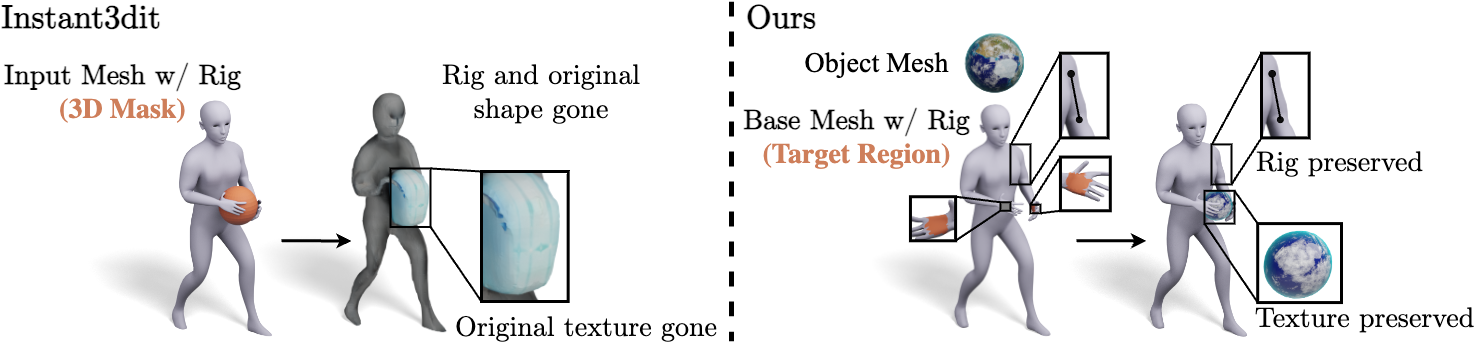
\includegraphics[width=\textwidth]{figures/instant3dit_comparison/instant3dit_comparison.png}
    \captionof{figure}{Digital artists often load shapes from pre-existing libraries of meshes that include additional information like animation rigs, skinning weights, texture maps and more. Generative shape editing methods like Instant3dit \cite{barda2025instant3dit} discard this information, performing global changes to the shapes and merging them together. \ourmethod{} is designed to fit exactly within this common artistic pipeline, and perfectly preserves all pre-existing information on the input meshes.}
    \label{fig:instant3dit_comparison}
    \vspace{-5.9mm}
\end{figure*}%
